\documentclass{article}

% General package includes
\usepackage{amsmath}
\usepackage{amssymb}
\usepackage{amsfonts}
\usepackage{mathtools}
\usepackage{fontspec}
\usepackage{changepage}
\usepackage{todonotes}
\usepackage{mathpartir}
\usepackage{mdframed}
% needed for some symbols in Iris
\usepackage{stmaryrd}
\usepackage{array}
\usepackage{makecell}
\usepackage{cancel}
\usepackage{xcolor}
\usepackage{longtable}
% \usepackage{tcolorbox}

% Moving figure captions closer to the contents.
\usepackage[skip=3pt]{caption}

% Styling links
\usepackage{hyperref}
\hypersetup{
    %colorlinks=true,
    linkcolor=black,
    citecolor=black,
    %filecolor=magenta,      
    urlcolor=blue,
    % frenchlinks=true
    }
\urlstyle{same}

% For bibliography
\usepackage{biblatex}
\addbibresource{thesis.bib}

% Settings page size
\usepackage{geometry}
\geometry{a4paper, margin=3cm}

% For including images
\usepackage{graphicx}
% https://www.overleaf.com/learn/latex/Inserting_Images#The_folder_path_to_images
\graphicspath{{./images/}}

% Font configuration
\usepackage[
    math-style=ISO,
    bold-style=ISO,
    partial=upright,
    nabla=upright
]{unicode-math}

\setmainfont{Libertinus Serif}
\setsansfont{Libertinus Sans}
\setmathfont{Libertinus Math}
\setmonofont{Source Code Pro}
\newfontfamily\symfont{FreeMono}
\newfontfamily\symfontextra{FreeSerif}

% Define some unicode characters missing from Source Code Pro
\usepackage{newunicodechar}
\newunicodechar{∗}{{\symfont ∗}}
\newunicodechar{⊥}{{\symfont ⊥}}
\newunicodechar{⊤}{{\symfont ⊤}}
\newunicodechar{▷}{{\symfont ▷}}
\newunicodechar{↦}{{\symfont ↦}}
\newunicodechar{∨}{{\symfont ∨}}
\newunicodechar{∈}{{\symfont ∈}}
\newunicodechar{γ}{{\symfont γ}}
\newunicodechar{Φ}{{\symfont Φ}}
\newunicodechar{⊢}{{\symfont ⊢}}

  
% For including source code blocks
\usepackage{minted}
\usepackage{xpatch}
% Remove latex indent for source code
\setminted{autogobble,linenos,fontsize=\footnotesize}
% Define inline shortcuts without syntax highlighting
\newmintinline[ocamlin]{text}{fontsize=\footnotesize}
\newmintinline[ocamlreal]{ocaml}{fontsize=\footnotesize}
\newmintinline[coqin]{text}{}
% disable comments using italics
% from https://tex.stackexchange.com/a/469702
\xpatchcmd{\minted}{\VerbatimEnvironment}{\VerbatimEnvironment\let\itshape\relax}{}{}

\BeforeBeginEnvironment{minted}{\begin{mdframed}}
\AfterEndEnvironment{minted}{\end{mdframed}}

% Iris/separation logic definitions
\usepackage{iris}

% Some custom shortcuts
\newcommand{\hazel}{Hazel}
\newcommand{\ocf}{OCaml~5}
\newcommand{\done}{{\symfontextra ✓}}
\newcommand{\tbd}{{\symfontextra ⌛}}
\newcommand{\efork}{\emph{Fork}}
\newcommand{\esuspend}{\emph{Suspend}}
\newcommand{\egetctx}{\emph{GetContext}}
\newcommand{\proto}{\emph{Coop}}
\newcommand{\protod}{\emph{Coop}~\ensuremath{\delta}}
\newcommand{\gsIsReg}{\emph{isRegister}}
\newcommand{\gsIsWaker}{\emph{isWaker}}
\newcommand{\gsIsCb}{\emph{isCallback}}
\NewDocumentCommand\ewp{O{} m O{} m m}%
  {\mathit{ewp}^{#1}_{#3}\spac\left(#2\right)\spac\left\langle#4\right\rangle\spac{\left\{#5\right\}}}
\newcommand{\ewpt}{\emph{ewp}}
\newcommand{\gsReady}{\emph{Ready}}
\newcommand{\gsPState}{\emph{PromiseState}}
\newcommand{\gsPInvIn}{\emph{PInvInner}}
\newcommand{\gsPInv}{\emph{PromiseInv}}
\newcommand{\invN}{\ensuremath{\mathcal{N}}}
\newcommand{\gsFiberResources}{\emph{fiberResources}}
\newcommand{\gsIsFiberContext}{\emph{isFiberContext}}
\newcommand{\gsTLVAg}{\emph{tlvAg}}
\newcommand{\gsSavedPred}{\emph{savedPred}}
\newcommand{\gsIsPr}{\emph{isPromise}}
\newcommand{\gsIsQueue}{\emph{isQueue}}
\newcommand{\gsIsBcst}{\emph{isBroadcast}}
\newcommand{\gspwait}{\emph{promiseWaiting}~\ensuremath{\gamma}}
\newcommand{\gspdone}{\emph{promiseDone}~\ensuremath{\gamma}}
\newcommand{\gssignal}{\emph{signalAllPermit}}
% A variable number of quads
% https://tex.stackexchange.com/a/330591
\newcommand{\myquad}[1][1]{\hspace*{#1em}\ignorespaces}

\title{Verifying an Effect-Based Cooperative Concurrency Scheduler in Iris}
\author{
    Adrian Dapprich \\
    Department of Computer Science\\
    Saarland University \\\\
    Advisors: Prof. Derek Dreyer \& Prof. François Pottier}
% \institute{Foundations of Programming Group, MPI-SWS, Saarland University}
\date{\today}

\begin{document}

% TODO better title page
\maketitle
\newpage

\tableofcontents
\newpage

\section{Introduction}
\label{sec:introduction}

\paragraph{}
With the spread of the Internet and computers transmitting ever more data there has been a trend in programming languages to support \emph{user-level concurrency} constructs
where an application is responsible to schedule the execution of multiple \emph{tasks} (i.e. some unit of work), analogous to how an operating system traditionally schedules multiple processes.
User-level concurrency is especially beneficial when there are many small tasks that are often blocked until an I/O resource like a network socket becomes available (i.e. they are \emph{I/O bound}).
In this case the application can quickly switch to another task that is able to do work, avoiding costly jumps to kernel code and doing a context switch.
Another advantage is that user-level concurrency has a lighter memory footprint.
This way an application can organize many more tasks (possibly on the order of millions) than if it uses a traditional thread-per-task approach.

There is not one standardized implementation for user-level concurrency.
It is generally said to use \emph{lightweight threads} as opposed to operating system threads, but in different languages or language libraries the concept is known under terms
like \emph{async/await} (Rust, Python, Javascript), \emph{goroutines} (Go), and \emph{fibers} (Java's Project Loom, \ocf{}'s Eio).

\paragraph{}

In this thesis we look at the Eio library of \ocf{} and formally verify the safety of its core elements for user-level concurrency.
The library uses the new effect handler feature~\cite{?} from \ocf{} to implement fibers in an efficient way without stack copying~\cite{?}.
In order to formally verify the code that uses effect handlers we use the \hazel{} program logic by de Vilhena~\cite{de2021separation,de2022proof}.

\paragraph{Formal Verification}
There is a growing need for the formal verification of programs or computer systems to provide a high assurance that they are "safe to use".
Formal verification means mathematically modelling programs to enable rigorous proofs about their properties.
As such, it also entails mathematically defining when a program is "safe to use".
Two important concepts behind this intuition are \textbf{safety} and \textbf{functional correctness}.
By safety, we mean that when evaluating a given program according to the rules of the language
it will never get into a state where there are no rules of how to evaluate it further.
In some languages this is called \emph{undefined behavior}, but we often model it as crashing the program.
Safety is the baseline for the type of program verification that we do and as a next step we can show that programs are functionally correct by proving that they obey a \textbf{specification}.
Specifications further restrict the possible program executions to a defined set of "good behaviors", such as "for a given input \(n\), this program computes the \(n\)th Fibonacci number".

\paragraph{Separation Logic}
We express specifications as logical propositions and do all reasoning in a separation logic called \emph{Iris}~\cite{jung2018iris}.
Separation logics~\cite{?} are based on Hoare logic, which has the \emph{Hoare triple} construct \(\{P\}\,s\,\{Q\}\) to encode the specification of a program.
It means that given preconditions \(P\), execution of the program \(s\) either diverges or terminates so that the postcondition \(Q\) holds\footnote{We only look at expression-based languages where \(Q\) is allowed to mention the final value of \(s\).}.
Further, separation logics are a type of affine logic that have a \emph{separating conjunction} connective \(P \ast Q\) in addition to the standard logical connectives.

The separating conjunction allows an interpretation of propositions as \emph{resources} that can be split up into disjoint parts \(P\) and \(Q\).
The most prominent example of a resource is the proposition \(l \mapsto v\) (also called \emph{points-to connective}), representing a heap fragment where the location \(l\) holds the value \(v\).
This also implies \emph{ownership} over the location \(l\), i.e. no one else can access the location as long as we have that resource.
A separating conjunction of heap fragments \(l \mapsto v \ast l' \mapsto v'\) additionally implies that \(l \neq l'\), because the heap fragments are necessarily disjoint.
The dual connective of a separating conjunction is the \emph{magic wand} \(P \wand Q\), which follows the elimination rule \(P \ast (P \wand Q) \vdash Q\).

Another type of proposition is duplicable \emph{knowledge}, which is also called \emph{persistent}.
For example, Hoare triples \(\{P\}\,s\,\{Q\}\) are defined as persistent because under the given assumptions \(P\) the evaluation of \(s\) should always be valid.
Separation logics have been successfully applied in many program verification developments~\cite{?,?,?} as they are useful for modular reasoning about stateful and multithreaded programs.

\paragraph{Iris}
Iris is not only a separation logic, but a whole separation logic framework implemented in Coq that can be instantiated with different programming languages.
This allows us to layer different \emph{program logics} on top of the base separation logic, which contain additional reasoning rules about the evaluation of programs in a concrete language.
Verifying a program in Iris follows the schema of first deciding which specifications are necessary for each of the program's components.
These are expressed using predicates in the logic, which we call the \emph{logical state definitions}.
If necessary, one can also use so-called \emph{ghost state},
which is a versatile feature of Iris that allows keeping track of program state and mutating it during a proof.
For complicated programs we often define ghost state and derive additional rules that modify it, in order to model the complex state space and state transitions of the program execution.
Ghost state updates in Iris are restricted to happen under an \emph{update modality} \(\upd P\).

The last step in proving the program specification consists of deriving a (partial) \emph{weakest precondition} \(\wpre{e}{v.\, Q\, v}\) for the program expression \(e\).
The weakest precondition is defined such that, if evaluation of \(e\) eventually terminates (i.e. divergence is permitted) in a final value \(v\), it must satisfy \(Q\; v\).
The name is derived from the fact that it is by definition the weakest precondition \(P\) that makes the Hoare triple \(\{P\}\,e\,\{v.\,Q\,v\}\) true.
Hoare triples are even defined this way in Iris:
\[
    \{P\}\,e\,\{v.\,Q\,v\} \coloneq \always (P \wand \wpre{e}{v.\, Q\, v})
\]
Since propositions are affine by default, the \emph{persistence modality} \(\always P\) is used to define Hoare triples as persistent.
Therefore, deriving a weakest precondition for an expression \(e\) proves a specification for it in terms of the assumptions \(P\) and conclusion \(Q\).
This also establishes the safety of the expression due to a soundness lemma of the logic.

One other powerful feature of Iris are \emph{shared invariants} \(\knowInv{\mathcal{N}}{I}\), which represent knowledge that a resource does not change over time, so they are also persistent.
They are used to encapsulate a resource \(I\) in order to share it under the restriction that the invariant can only be opened for one atomic step of execution at a time.
If the invariant is opened, the contained resource \(I\) can be accessed but must be restored at the end of the execution step.
This ensures that even in the presence of multiple threads executing in parallel, the invariant is never observably violated.

The standard language for Iris is called heaplang and is an ML-type language with mutable state and multithreading.
However, it does not support effect handlers as present in \ocf{}.
So for reasoning about programs with effect handlers we use the \hazel{} language for Iris.

\paragraph{Effect Handlers}
\emph{Effect handlers}~\cite{plotkin2013handling} (and the related concept of \emph{algebraic effects}) are a versatile concept explored in some research languages~\cite{eff,koka} and now also implemented in \ocf{}~\cite{ocamleff}.
They are often called \emph{resumable exceptions} because analogous to exception handlers, one installs an effect handler around an expression \ocamlin{e} to handle its effects,
but the effect handler also receives a delimited continuation \ocamlin{k}, representing the rest of the computation of \ocamlin{e} from the point where the effect was performed.
The \ocf{} implementation brings with it an extensible variant type \ocamlin{eff}, meaning one can add new constructors to the type to define effects, and a keyword \ocamlin{perform} to perform an effect,
which transfers control to an appropriate effect handler.

We present code examples in a simplified \ocf{} syntax\footnote{This syntax is planned to be implemented in \ocf{} in the future: \url{https://github.com/ocaml/ocaml/pull/12309}}
as shown in figure~\ref{fig:effect-example}, because the concrete syntax of effect handlers is verbose.
We use an overloading of the \ocamlin{match} expression, which includes cases for handled effects, that is common in the literature.

\begin{figure}[ht]
    \begin{minted}[fontsize=\footnotesize,escapeinside=@@]{ocaml}
    (* Declares a new constructor for the effect type 
     * E : int -> bool Effect.t *)
    type _ eff += E : int -> bool eff

    (* Evaluating a perform expression with a value of type 'a Effect.t 
     * transfers control to the enclosing handler and (possibly)
     * terminates in a value of type 'a. *)
    let e () = 
      let (b : bool) = perform (E 1) in
      b

    (* Evaluates the expression e () and if the effect E is performed,
     * control is transferred to the second branch.
     * The match acts as a deep handler, i.e. even if during the 
     * evaluation of e the effect E is performed multiple times, the
     * second branch is evaluated every time.
     * When e is reduced to a value, the non-effect branches are 
     * used for pattern matching as usual. *)
    match e () with
    | v -> v
    (* This handler just checks if the passed value is 1.
     * Applying k to a value adds the continuation to the stack,
     * so control is transferred back to where the perform expression 
     * was evaluated. *)
    | @\texttt{\textbf{effect}}@ (E v) k -> k (v = 1)
\end{minted}
    \caption{Example for the effect handler syntax.}
    \label{fig:effect-example}
\end{figure}

The biggest advantage of effect handlers for treating effects in a language over using monads is that they are more composable.
For one, using non-monadic functions together with monadic functions often requires rewriting parts of the code into monadic style.
Also, composing multiple monads results in monad transformer stacks which are notoriously confusing.
Instead, effect handlers can be layered just like normal exception handlers and code written without the use of effect handlers can be used as-is.

Languages like Koka additionally track the possible effects of an expression in their type.
This might be implemented for \ocf{} in the future, but for now effects are not tracked by the type system.
It is the responsibility of the programmer to install effect handlers that handle all possible effects of their program.
This raises the question of \textbf{effect safety} for OCaml programs using effect handlers, which means that a program does not perform any unhandled effects.
The \ocf{} runtime treats unhandled effects as an error and crash the program.
So to prove the safety of \ocf{} programs we must additionally establish their effect safety.

\paragraph{\hazel{} \& Protocols}
In our development we use the Iris language \hazel{} by de Vilhena~\cite{de2021separation,de2022proof} which formalizes an ML-like language with effect handlers.
We restate the most important concepts but for a deeper understanding we recommend reading~\cite{de2021separation}.

\hazel{} defines an \emph{extended weakest precondition} \(\ewp{e}{\Psi}{v,\, Q\, v}\) which -- in addition to what is implied by a normal weakest precondition --
shows we can observe that the expression \(e\) performs effects according to the protocol \(\Psi\).
A protocol \(\Psi\) acts as a specification for effects in terms of their "input" and "output", casting them in a similar light to function calls.
The main way to specify a protocol is by the following constructor.
\[
    !\, \overrightarrow{x}\, (v)\, \{P\}.\; ?\, \overrightarrow{y}\, (w)\, \{Q\}
\]
The input (!) and output (?) syntax is inspired by session types~\cite{sestypes} which are used to describe the behavior of communicating parties.
Intuitively, the part after the exclamation mark gets "sent" to the effect handler and the part after the question mark is "received" as an answer.
\(\overrightarrow{x}\) and \(\overrightarrow{y}\) are binders whose scope extends from their position all the way to the right.
The client who performs the effect transmits the value \(v\) to the effect handler and must prove the proposition \(P\).
In return, the client receives from the effect handler a value \(w\) and gets to assume \(Q\).
In total, this can be thought of as an analogue to a Hoare triple like \(\{P\}\, handler\; v\, \{w.\; Q\; w\}\), where we explicitly name the handler that handles the effect.
But the client only indirectly invokes the effect handler by evaluating a \(perform\) expression, so in practice we prove the following Hoare triple.
\[
    \{P\}\, perform\; v\, \{w.\; Q\; w\}
\]

Apart from the above there are three additional ways to define protocols.
There is the sum constructor \(\Psi_1 + \Psi_2\) to combine two protocols, allowing \(e\) to perform effects according to both, and its neutral element, the empty protocol \(\bot\),
which allows no effects.
Finally, there is a tag constructor \(\mathcal{f} \mathop{\#} \Psi\) to give a name to protocols.
Our example effect \ocamlin{E} from figure~\ref{fig:effect-example} could therefore be formalized using the following protocol \(\Psi_\mathtt{E}\).\todo{maybe more expressive example}
\[
    \Psi_\mathtt{E} \coloneq \mathtt{E} \mathop{\#}\; !\, i\, (i)\, \{ i \in \mathtt{int} \}.\; ?\, b\, (b)\, \{ b \in \mathtt{bool} \}
\]

Using the extended weakest precondition with the \(\bot\) protocol then enables us to prove that a program is \textbf{effect safe}, as it shows that we cannot observe any effects from the top level.
Note that internally the program can of course perform effects, but an effect handler hides the effects of its discriminant expression which leads to an empty protocol at the top.

\subsection{The Eio Library}
\label{sec:intro-eio}

We first give a general overview of the functionality provided by the Eio library before discussing what we focus on in our verification work in the next section.
Eio is a library for cooperative user-level concurrency where individual tasks are represented by \emph{fibers}\footnote{Note that these are technically different from the existing fiber concept in \ocf{}, where a fiber denotes a stack frame under an effect handler, and the runtime stack is a linked list of those fibers. But since Eio fibers are evaluated under an effect handler, they all have an associated OCaml fiber. See also: \url{https://v2.ocaml.org/manual/effects.html\#s:effects-fibers}}.
Fibers are just OCaml functions that are allowed to perform a defined set of effects to interact with the cooperative scheduler.
A scheduler is responsible for running an arbitrary amount of fibers in a single thread.
However, if multithreading is required it is possible to spawn additional schedulers in new threads, providing some initial fiber.

In a cooperative user-level concurrency setting, many existing APIs for operating system resources in OCaml are not suitable anymore because they are blocking.
Therefore, Eio also provides concurrency-aware abstractions to these resources, such as network sockets, the file system, and timers, i.e. they suspend the running fiber instead of blocking the system-level thread.
Since these schedulers must interact with operating system, there are specialized schedulers for multiple platforms such as Windows, Linux, and a generic POSIX scheduler.
Eio also offers synchronization and message passing constructs like mutexes and channels which are also concurrency-aware.

\subsection{Focus and Structure of the Thesis}
\label{sec:intro-structure}

Eio aims to be the standard cooperative concurrency library for \ocf{},
so it includes many functions implementing structured concurrency of fibers (e.g. \ocamlin{Fiber.{first, any, both, all}}, which run two or more fibers and combine their results),
support for cancelling fibers, abstractions for operating system resources,
a different scheduler implementation per platform, and synchronization constructs like promises and mutexes.
But for this work we restrict ourselves to verifying the safety and effect safety of Eio's core functionalities:
\begin{enumerate}
    \item Running fibers in a "common denominator" scheduler that does not interact with any operating system resources but just schedules fibers.
    \item Awaiting the result of other fibers using the \emph{promise} synchronization construct.
    \item And spawning new schedulers to run fibers in another thread.
\end{enumerate}

\begin{figure}[ht]
    \centering
    \includegraphics[width=0.75\textwidth]{Eio_Module_Hierarchy.png}
    \caption{Eio module hierarchy.}
    \label{fig:eio-module-hierarchy}
\end{figure}

Figure~\ref{fig:eio-module-hierarchy} shows the simplified module hierarchy of the concepts we focus on.
A standard arrow stands for a direct source code dependency from one module to another.
The diamond arrow between \ocamlin{Scheduler} and \ocamlin{Fiber} stands for the implicit dependency that fibers perform effects which are handled by code in the scheduler module.

Fibers can fork off new fibers using the \efork{} effect, suspend execution using the \esuspend{} effect, and get access to some context data using the \egetctx{} effect,
all of which are handled by the scheduler they are running in.
The implementation of the fiber and scheduler functions are discussed in section~\ref{sec:sched-impl}.
\emph{Promises} are built on top of the \emph{broadcast} data structure, which is a lock-free signalling construct that is used by fibers to signal other fibers when they are done.
The specification of promises is discussed in section~\ref{sec:sched-spec}.
Broadcast is based on the \emph{CQS} data structure, whose specification is already verified using Iris~\cite{koval2023cqs}, but Eio customizes the implementation so we had to adapt the proof.
We discuss this process in section~\ref{sec:broadcast}.
Fibers in Eio also have access to \emph{thread-local variables} by performing a \egetctx{} effect, which is discussed in section~\ref{sec:thread-local-vars}.
They are thread-local in the sense that they are shared between all fibers of one scheduler.
Finally, we discuss our addition of multithreading to the \hazel{} operational semantics in order to model running schedulers in different threads.
This turned out to be technically trivial, so we only discuss it in appendix~\ref{sec:apdx-mt} and take a multithreaded semantics and support for Iris \emph{shared invariants} as a given in the reminder of the main text.

\subsection{Contributions}
\label{sec:intro-contributions}

To summarize our contributions, in this thesis we verify the \textbf{safety} and \textbf{effect safety} of a simplified model of Eio which serves as an extended case study on the viability of \hazel{} for verifying programs with effect handlers.
This includes:

\begin{itemize}
    \item The verification of the basic Eio \textbf{fiber abstraction} running on a common denominator scheduler.
    \item Proving reusable specifications for the main three effects of Eio: \efork{}, \esuspend{}, and \egetctx{}.
    \item An adaptation of the existing verification of CQS to the customized version used by Eio.
    \item Adding multithreading to \hazel{}'s operational semantics, which shows we can reason about programs that use both \textbf{multithreading} and \textbf{effect handlers}.
\end{itemize}

\section{Verifying a Simplified Eio Scheduler}
\label{sec:scheduler}

\todo{mention that all code examples are an OCaml rendering of the verified Hazel code, based on but not equal to the Eio code}

Cooperative concurrency schedulers are commonly treated in the literature on effect handlers~\cite{dolan2018concurrent,leijen2017structured,de2021separation} because they are a lucid example for the usefulness of handling delimited continuations in this way.
Generally, the scheduler contains an effect handler and a fiber is just a normal function.
The fiber can yield execution by performing an effect, jumping to the effect handler (i.e. the scheduler) and providing it with the rest of the fiber's computation in the form of a continuation.
The scheduler has a collection of continuations and by invoking one of them it schedules the next fiber.
This approach is also used in Eio.

We can therefore use the simple cooperative concurrency scheduler case study from the dissertation of de Vilhena~\cite{de2022proof} as a starting point for our verification work.
In the following section we discuss the implementation of the simplified Eio model in more detail.
Using the implementation we give an intution about what specifications the functions should satisfy and what kind of logical state is needed to prove these specifications.
On this intuition we will then build a formalization in section~\ref{sec:sched-spec}.
% But some key differences in the implementation of Eio allow simplifications of the logical state that we use in our proofs. 

\subsection{Implementation}
\label{sec:sched-impl}

Let us first get an idea of how different components of the core Eio fiber abstraction interact by looking at their types.
\ocamlin{Scheduler.run}\footnote{The scheduler's result is optional because the main fiber might deadlock.} is the main entrypoint to Eio and it is provided a function which represents the first fiber to be executed.
The scheduler runs the main fiber and all forked-off fibers in a single thread.
However, a fiber can also spawn new schedulers in separate threads to run other fibers in parallel as explained in~\ref{sec:apdx-mt}
\ocamlin{Fiber.fork_promise} is also provided a function which represents a fiber, but this one will be forked in the current scheduler so that it runs concurrenctly.
It returns a promise holding the eventual return value of the new fiber.
The promise is thread-safe so that also fibers running in different threads can use the \ocamlin{Promise.await} function to wait until the value is available.
Common problems like deadlocks are not prevented in any way and are the responsibility of the programmer.
% The function sends the fiber to the scheduler by performing an effect, so it must always be called from a fiber itself.


\begin{minted}{ocaml}
    Scheduler.run : (() -> 'a) -> 'a option
    Fiber.fork_promise : (() -> 'a) -> 'a Promise.t
    Promise.await : 'a Promise.t -> 'a
\end{minted}

We present code examples in a pseudo-\ocf{} syntax because the concrete syntax of effect handlers is verbose.
Instead, we use an overloading of the match syntax that is common in the literature which includes cases for handled effects.

\begin{minted}[fontsize=\footnotesize]{ocaml}
    (* declares an effect E that carries a value of type int and has a bool return value. *)
    effect E : int -> bool

    (* Matches on the expression e and evaluates the second branch if it performs the effect E.
     * The continuation k captures the rest of the computation of e.
     * It acts as a deep handler, i.e. even if evaluating e performs E more than once the 
     * second branch will be evaluated every time. *)
    match e with
    | v -> ...
    | effect (E v) k -> ...
\end{minted}

\subsubsection{\ocamlin{Scheduler.run}}
\label{sec:sched-impl-run}

As mentioned above this is the main entry point to the Eio library.
It receives the main fiber as an argument and sets up the scheduler environment.

The \ocamlin{run_queue} contains closures that will immediately invoke the continuation of an effect.
This represents ready fibers which can continue execution from the point where they performed an effect.

The \ocamlin{next} function pops one fiber (i.e. function) from the \ocamlin{run_queue} and executes it.
If no more ready fibers remain -- either because all fibers terminated or there is a deadlock -- the next function just returns and the scheduler exits.

The inner \ocamlin{execute} function is called once on each fiber to execute it and handle any performed effects.
The return value of a fiber given to the \ocamlin{execute} function is always just unit.
\begin{itemize}
  \item The main fiber is wrapped in a closure that saves its return value in a reference and returns unit so that \ocamlin{execute} does not need to differentiate between the main fiber and any other fiber.
  \item All other fibers are forked using \ocamlin{Fiber.fork_promise}, which also wraps them in a closure that saves their return value in a promise and returns unit.
\end{itemize}

This emphasizes the fact that an Eio scheduler is only used for running fibers.
The interaction between fibers waiting for values of other fibers is handled separately in promises.

Handling a \efork{} effect is simple because it just carries a new fiber to be executed so the handler recursively calls the \ocamlin{execute} function to execute it immediately.
The execution of the original fiber is paused due to performing an effect and its continuation \ocamlin{k} is placed in the run queue so that it can be scheduled again.
This prioritizes the execution of a new fiber and is a design decision by Eio.
It would be equally valid to place the \ocamlin{fiber} argument in the run queue.

Handling a \esuspend{} effect may look complicated at first due to the higher-order \ocamlin{register} function.
This effect is used by fibers to suspend execution until some condition is met.
The fiber defines this condition by constructing a \ocamlin{register} function that in turn receives a wakeup capability by the scheduler in form of the \ocamlin{waker} function.
The key point is that as long as the continuation \ocamlin{k} is not invoked, the fiber will not continue execution.
So the \ocamlin{waker} function wakes up a fiber by placing its continuation into the run queue.
The \ocamlin{register} function is called by the scheduler right after the fiber suspends execution and can then install \ocamlin{waker} as a callback at a suitable place (or even call it directly).
For example, to implement promises, the \ocamlin{waker} function is installed in a datastructure that will call the function after the promise is fulfilled.

Note that the \ocamlin{waker} function's argument \ocamlin{v} has a \textit{locally abstract type}, which is a typical pattern in effect handlers.
From the point of view of the fiber, the polymorphic type of the \esuspend{} effect is instanitated depending on how the effect's return value is used.
But the scheduler does not get any information about this so the argument type of the continuation \ocamlin{k} and the \ocamlin{waker} function is still abstract.

Waking up should be possible across thread boundaries, which is why the run queue in Eio needs to be thread-safe.
For the verification we assume the specification of a suitable \ocamlin{Queue} module that supports thread-safe push and pop operations.

% <!-- In our simplified model of Eio, the `Suspend` effect is only performed in the implementation of `Promise.await` which registers the `waker` callback to be called when the promise is fulfilled. -->

\begin{minted}{ocaml}
effect Fork : (() -> 'a) -> ()
type 'a waker : 'a -> ()
effect Suspend : ('a waker -> ()) -> 'a

let run (main : () -> 'a) : option 'a =
  let run_queue = Queue.create () in
  let next () =
    match Queue.pop run_queue with
    | None -> ()
    | Some cont -> cont ()
  let rec execute fiber =
    match fiber () with
    | () -> next ()
    | effect (Fork fiber) k ->
      Queue.push run_queue (fun () -> invoke k ());
      execute fiber
    | effect (Suspend register) k =>
      let waker = fun v -> Queue.push run_queue (fun () -> invoke k v) in
      register waker;
      next ()
  in
  let result = ref None in
  execute (fun () -> result := main ());
  !result
\end{minted}

\subsubsection{\ocamlin{Fiber.fork_promise}}
\label{sec:sched-impl-fork}

This is the basic way to create a new fiber in Eio and the only one we model in our case study.
It will create a promise and spawn the provided function as a new fiber using the \efork{} effect.
When \ocamlin{f} is reduced to a value \ocamlin{result}, it will fulfill the promise with that value and signal all fibers waiting for that result to wake up.
The major difference to the implementation of de Vilhena is that promises in Eio are entirely handled by the fiber, and not in the effect handler code of the scheduler.
This achieves a better separation of concerns and simplifies the logical state needed for the proof.

\begin{minted}{ocaml}
let fork_promise (f : () -> 'a) : 'a Promise.t =
  let p = Promise.create () in
  let fiber = fun () ->
    let result = f () in
    match Atomic.get p with
    | Done _ -> error "impossible"
    | Waiting cqs ->
        Atomic.set p (Done result);
        CQS.signal_all cqs 
  in
  perform (Fork fiber) 
  p
\end{minted}

\subsubsection{\ocamlin{Promise.await}}
\label{sec:sched-impl-await}

This is the most complicated looking function in our case study which is partly due to the \esuspend{} effect and also due to the use of CQS functions.
The purpose of \ocamlin{Promise.await p} is to suspend execution of the calling fiber until \ocamlin{p} is fulfilled and then return its value.
The "suspend execution" part is handled by performing the \esuspend{} effect.
Then, the "until \ocamlin{p} is fulfilled" part is implemented by using CQS~\cite{koval2023cqs} functions as described in the following.

CQS is an implementation of the observer pattern and functionally similar to condition variables\footnote{\url{https://en.cppreference.com/w/cpp/thread/condition_variable}} in languages like C++ (as defined by the POSIX standard), allowing fibers to register callbacks that will be called when a condition is signalled.
The difference is that traditional condition variables are always used together with a mutex to enable synchronization between different threads, while CQS is a lock-free datastructure implementing a similar API.

Below we show the public API of the CQS module. The implementation and specification will be exapanded upon in section~\ref{sec:cqs}.
\begin{minted}{ocaml}
type callback = () -> ()
type register_handle

val create : () -> t
val register : t -> callback -> register_handle option
val try_cancel : register_handle -> bool
val signal_all : t -> ()
\end{minted}

In the \ocamlin{Promise.await} function if the promise is not fulfilled initially the fiber should wait until that is the case so it registers the \ocamlin{waker} function with CQS by using \ocamlin{CQS.register}.
In turn, the \ocamlin{Fiber.fork_promise} function is reponsible for fulfilling the promise and it uses \ocamlin{CQS.signal_all} to call all \ocamlin{waker} functions registered with CQS.
Recall that calling a \ocamlin{waker} function will enqueue the fiber that performed the \esuspend{} effect in the scheduler's run queue so that it can continue execution.
In the default case the following simplified chain of events is established:
\begin{enumerate}
  \item The fiber suspends execution at the point of evaluating \ocamlin{perform (Suspend register)}.
  \item The \ocamlin{waker} function is registed with CQS.
  \item The promise is fulfilled.
  \item The \ocamlin{waker} function is called.
  \item The fiber resumes execution at the point of evaluating \ocamlin{perform (Suspend register)}.
\end{enumerate}
Therefore, after the \esuspend{} effect returns we know the state of the promise is \ocamlin{Done} and the final value can be returned.

But because CQS is lock-free and promises can be shared between different threads there are a number of possible interleavings that the \ocamlin{register} function must take care of aswell.
The definition of the register function is interesting enough that we split it out into \ocamlin{make_register} and give a separate specification, even though it is not part of the public API of the module.
First, there could be a race on the state of the promise itself.
Right after the state is read in line 19 another thread might change the state to \ocamlin{Done} and go on to call \ocamlin{CQS.signal_all}.
If that happes there is another race between the \ocamlin{CQS.register} in line 7 and the \ocamlin{CQS.signal_all} in the other thread.
If \ocamlin{CQS.register} notices that there is a racing \ocamlin{CQS.signal_all} it will directly call the \ocamlin{waker}\footnote{TODO mention that this is just an optimization.}.
Otherwise, the \ocamlin{waker} is registered but in fact the \ocamlin{CQS.signal_all} might have already finished before \ocamlin{CQS.register} even started.
In this case the \ocamlin{waker} would be "lost" in the CQS, never to be called.
To avoid this, \ocamlin{register} must check the state of the promise again in line 12, and if it is fulfilled try to cancel the \ocamlin{waker} registration.
The cancel will fail if the \ocamlin{waker} function was already called.
If it succeeds the \ocamlin{register} function has the responsibility of calling \ocamlin{waker} itself.

\begin{minted}{ocaml}
type 'a t = Done of 'a | Waiting of CQS.t

let create () : 'a t = 
  let cqs = CQS.create () in
  Atomic.create (Waiting cqs)

let make_register (p: 'a t) (cqs: CQS.t) : (() waker -> ()) = 
  fun waker ->
    let register_result = CQS.register cqs waker in
    match register_result with
    | None -> ()
    | Some register_handle ->
      match Atomic.get p with
      | Done result ->  
        if CQS.try_cancel register_handle
        then waker ()
        else ()
      | Waiting _ -> ()

let await (p: 'a t) : 'a = 
  match Atomic.get p with
  | Done result -> result
  | Waiting cqs ->
    let register = make_register p cqs
    perform (Suspend register);
    match Atomic.get p with
    | Done result -> result 
    | Waiting _ -> error "impossible"
\end{minted}

The only \textbf{safety} concerns in the above implementation are \ocamlin{Fiber.fork_promise} expecting the promise to be unfulfilled and \ocamlin{Promise.await} expecting the promise to be fulfilled in the last match.
In both cases, the program would crash (signified by the \ocamlin{error} expression) if the expectation is violated.
So to establish the safety of Eio we wish to prove that the expectations always hold and the two \ocamlin{error} expressions are never reached.
In the next section we show how the first situation is addressed by defining a unique resource that is needed to fulfill a promise, and the latter is a consequence of the protocol of the \esuspend{} effect.

\subsection{Specification}
\label{sec:sched-spec}

To prove specifications for an effectful program in Hazel we have to define not only ghost state constructs to track program state as usual but also protocols which describe the behavior of the program's effects.
To use them in our Eio case study we adapt both the ghost state and the effect protocols from the cooperative concurrency scheduler case study from chapter 4 of de Vilhena's dissertation~\cite{de2022proof}

\subsubsection{Protocols}
\label{sec:sched-spec-protocols}

First we look at the protocols for the \efork{} and \esuspend{} effect.
In Hazels' protocol syntax they are formalized in the following way, where the precondition of \esuspend{} is given the name \isreg{} to describe the behavior of the fiber-defined \ocamlin{register} function.

\begin{figure}[ht]
  \begin{alignat*}{2}
    isRegister\; reg\; P & \Coloneqq   & \forall waker.\; ( & \forall v.\;  P\; v \wand{} \ewp{waker\; v}{\bot}{\top}) \wand{} \later \ewp{reg\; waker}{\bot}{\top} \\
    \proto{}             & \Coloneqq\; & \quad Fork\; \#    & \; !\; e\; (e)\; \{\later \ewp{e}{\proto{}}{\top}\}. ?\; ()\; \{ \top \}                              \\
                         &             & Suspend\;    \#    & \; !\; reg\; P\; (reg)\; \{isRegister\; reg\; P\}.?\; y\; (y)\; \{ P\; y \}
  \end{alignat*}
  \caption{Definition of \proto{} Protocol with \efork{} \& \esuspend{} Effects.}
  \label{fig:coop-protocol-simpl}
\end{figure}

The \efork{} effect stays almost the same compared to de Vilhena's case study.
It accepts an arbitraty expression \ocamlin{e} which represents the computation that a new fiber executes.
To perform the effect one must prove that \ocamlin{e} acts as a function that can be called on \ocamlin{()} and obeys the \ocamlin{Coop} protocol itself.
This means spawned off fibers can again perform \efork{} and \esuspend{} effects.
The \(\ewp{e}{\proto{}}{\top}\) is guarded behind a later modality because of the recursive occurrence of the \proto{} protocol.
Since promise handling is done entirely in the fibers and the effect just hands off the fiber to the scheduler, the protocol is simplified in two ways compared to the original.
First, the scheduler does not interact with the return value of the fiber so the \ewpt{} has a trivial postcondition.
Second, because the scheduler does not create the promise, the protocol itself also has a trivial postcondition.

The protocol for \esuspend{} is entirely new.
From the type of the \esuspend{} effect we already know that some value can be transmitted from the party that calls the \ocamlin{waker} function to the fiber that performed the effect.
The protocol now expresses the same idea on the level of resources.
To suspend, a fiber must supply a function \ocamlin{register} that satisfies the \isreg{} predicate.
This predicate says that \ocamlin{register} must be callable on a \ocamlin{waker} function and in turn gets to assume that the \ocamlin{waker} function is callable on an arbitrary value \ocamlin{v}, which satisfies the predicate \ocamlin{P}.
Both must not perform effects.
The predicate \ocamlin{P} appears twice in the definition of the protocol, once in the precondition of \ocamlin{waker} and then in the postcondition of the whole protocol.
It signifies the resources that are transmitted from the party that calls the \ocamlin{waker} function to the fiber that performed the effect.

By appropriately instantiating \ocamlin{P}, we can enforce that some condition holds before the fiber can be signalled to continue execution and we get to assume the resources \ocamlin{P v} for the rest of the execution.
For example, in the \ocamlin{Promise.await} specification below, we ensure that the promise must be fulfilled before the effect returns by instantiating \ocamlin{P} with a resource that says the promise is fulfilled.

\subsubsection{Logical State}
\label{sec:sched-spec-state}

The most basic ghost state we track is wether a promise is fulfilled or not.
If a promise \ocamlin{p} is unfulfilled, two copies of \gspwait{} exist\todo{maybe use meta\_tokens to hide gamma}, one owned by the fiber and one by the invariant that tracks all promises.
When fulfilling the promise, both copies can be combined and converted to a persistent \gspdone{} resource.
The \gspwait{} and \gspdone{} resources cannot exist at the same time.
This design allows us to deduce the current state of the promise depending on if we own a \gspwait{} or a \gspdone{}.
This is formalized in the rules in figure~\ref{fig:promise-state-rules}.

\begin{figure}
  \caption{Logical Rules for the \textit{Promise State} Resource}.
  \label{fig:promise-state-rules}
\end{figure}

The resource \gsPInv{} tracks the state of all existing promises by using an authoritative map which contains for each promise: a location \ocamlin{p} holding its current value, a ghost name \ocamlin{γ} that is used for the \gspwait{} and \gspdone{} resources, and a predicate \(Φ\) that describes the value the promise will eventually hold.
Additionally, for each promise in the map we own some resources as part of \gsPInv{} that depend on the current state of the promise.

As long as the promise is not fulfilled we own a broadcast, one copy of \gspwait{}, and a \gssignal{}.
The \gssignal{} is used to call the \ocamlin{CQS.signal_all} function which must only be called once.
When the promise has been fulfilled, we instead own a \gspdone{} and the knowledge that the final value satisfies the given postcondition \(Φ\).

The \gsReady{} predicate expresses that \textit{f} is safe to be executed and is used as the invariant for a scheduler's run queue, i.e. it should hold for all fibers in the run queue that they can be executed.


\begin{figure}[ht]
  \begin{align*}
    \gsPInv{}  \Coloneqq\;     & \exists M.\; isPromiseMap\; M \ast                                                                                                                        \\
                               & \quad \forall (p, \gamma) \mapsto \Phi \in M.\;                                                                                                           \\
                               & \qquad (\exists v.\; p \mapsto Done\; v \ast \texttt{promise\_done}\; \gamma \ast \always \Phi\; v)                                                       \\
                               & \quad \vee (\exists cqs.\; p \mapsto Waiting\; cqs \ast \texttt{is\_cqs}\; cqs \ast \texttt{promise\_waiting}\; \gamma \ast \texttt{signal\_all\_permit}) \\
    \gsReady{}\; f \Coloneqq\; & \ewp{f\; ()}{\bot}{\top}
  \end{align*}
  \caption{Logical State Definitions for the Verification of Scheduler \& Promise Modules}
  \label{fig:logical-state-simpl}
\end{figure}

\begin{figure}[ht]
  \begin{align*}
    TODO\; combine promise waiting, contradiction for promise waiting and done, lookup promise, ...
  \end{align*}
  \caption{Derived Rules about the Logical State}
\end{figure}

\subsubsection{Comparison of Logical State}
\label{sec:sched-spec-state-comparison}

\todo{insert logical state from the dissertation}

In de Vilhena's case study, the \gsReady{} predicate fulfills two roles.
\begin{enumerate}
  \item It expresses that all continuations in the scheduler's run-queue are safe to execute.
  \item It expresses that all continuations in a promise's waiting-queue are safe to execute.
\end{enumerate}

It was necessary to have both \gsPInv{} and \gsIsQueue{} as preconditions because they describe global state so they had to be passed around.

In our case study \gsPInv{} was dropped from the definition of Ready because it is now put into an Iris shareable invariant, so we don't need to pass it around explicitly.
Similarly, the isQueue precondition was dropped from the definition of Ready because in Eio the run queue must be thread-safe, so our new isQueue is persistent and we don't need to pass it around explicitly.
Therefore, our \gsReady{} is neither recursive nor mutually recursive with \gsPInv{} anymore, which simplifies its usage in Iris.
We note that the (mutual) recursion was only necessary because \gsPInv{} was used to track global state but was not put into an Iris shareable invariant, so it had to be passed around explicitly in many places.

We also split up the two uses of \gsReady{} and only use it under this name for the first role.
In the case of a scheduler's run-queue the \ocamlin{Φ v} degenerates just to \ocamlin{v = ()}, so we can drop both from the definition and use \ocamlin{()} directly.
This is why in our definition of \gsReady{} it is only an \ewpt{} without preconditions.

For the second use case of describing the continuations in a promise's waiting-queue we now have another specialized version of \gsReady{}.
A broadcast has the following invariant for all stored callbacks: \ocamlin{P v -∗ ewp (callback ()) <| ⊥ |> {{ ⊤ }}}.
This is just \gsReady{} where \ocamlin{P v} replaces \ocamlin{Φ v}, which is the same \ocamlin{P} as in the definition of the \esuspend{} effect since the callbacks in a broadcast are \ocamlin{waker} functions.

\subsubsection{\ocamlin{Scheduler.run}}
\label{sec:sched-spec-run}

The interesting part about the scheduler specification is that it proves \textbf{effect safety} of the runtime, i.e. no matter what a fiber does it will not crash the scheduler due to an unhandled effect.
However, the specification only talks about effect safety and not about handling fibers correctly in any other way, e.g. regarding fairness of scheduling or just not dropping fibers.
For example, a trivial function which ignores the \ocamlin{main} argument and immediately returns satisfies the same specificaiton.
For a scheduler it would be desirable to prove these properties, too, but since they are liveness properties it is hard to do in Iris and not a focus of this thesis.

\begin{minted}{coq}
Lemma ewp_run (main : val) :
  EWP main #() <| Coop |> {{ ⊤ }} -∗
    EWP run main <| ⊥ |> {{ ⊤ }}.
\end{minted}

The proof proceeds as follows:
- Creating the run queue also returns a persistent resource which is used for all later calls to the \ocamlin{next} function.
- For the inner \efork{} function we use Löb induction since it is called recursively.
- Since it is a deep effect handler we need to satisfy the \ocamlin{deep-handler} predicate for the \ocamlin{Coop} protocol.
- The \efork{} case just recurses in the \efork{} function so we use the induction hypothesis.
- For the \esuspend{} case we define the \ocamlin{waker} function and prove \ocamlin{P v -∗ EWP waker () <| ⊥ |> {{ ⊤ }}} in order to call the \ocamlin{register} function on it.
This holds by construction of the \ocamlin{waker} function because \ocamlin{P v} is a precondition for invoking the fiber's continuation \ocamlin{k}.

\subsubsection{\ocamlin{Fiber.fork_promise}}
\label{sec:sched-spec-fork}

For this specification, the \gsPInv{} argument is needed to interact with promises and the \ewpt{} proves that the new fiber is safe to execute and obeys the \ocamlin{Coop} protocol.
In return, the caller gets a promise that will eventually hold a value satisfying the predicate \(Φ\).

\begin{minted}{coq}
Lemma ewp_fork_promise (f: val) Φ :
  promiseInv ∗ EWP f #() <| Coop |> {{v, □ Φ v}}
⊢ 
  EWP (fork_promise f) <| Coop |> {{ y, 
    ∃ (p: loc), ⌜ y = #p ⌝ ∗ isPromise p Φ}}.
\end{minted}

The proof proceeds as follows:
- First, a new promise is created, which updates the \gsPInv{} invariant and yields one half of the \gspwait{} resource for that new promise.
- We define the actual fiber and prove its \ewpt{}.
- Evaluating \ocamlin{f} yields a value satisfying \(Φ\) as given by the \ewpt{}.
- Because we own \gspwait{} the second branch of the match can be ruled out. Now the \gsPInv{} invariant is accessed to update the promise state to \ocamlin{Done}. This consumes both halves of the \gspwait{} resource and yields a \gspdone{}. We also take out the \gssignal{}.
- We use this permit along with \gspdone{} to call \ocamlin{CQS.signal_all}. \gspdone{} is persistent so it can be used to call all wakers.
- Using the \ewpt{} for the wrapped \ocamlin{f} we can perform a \efork{} effect.
- Since the promise will be fulfilled with a value satisfying \(Φ\) we have the \ocamlin{isPromise p Φ} that we must return.

\subsubsection{\ocamlin{Promise.await}}
\label{sec:sched-spec-await}

The implementation of \ocamlin{Promise.await} is very different from the original but still satisfies the same specification. \gsPInv{} and \textit{IsPromise} are both needed to interact with the promise's state.

\begin{minted}{coq}
Lemma ewp_await_make_register (p: loc) (cqs: val) Φ:
  isPromise p Φ ∗ is_cqs cqs 
⊢
  EWP (make_register #p cqs) <| ⊥ |> {{register, 
    ∀ (waker: val), (promise_done γ -∗ EWP waker #() <| ⊥ |> {{ ⊤ }}) -∗
    promiseInv -∗ 
      ▷ EWP register waker <| ⊥ |> {{ ⊤ }} }}.

Lemma ewp_await (p: loc) Φ :
  promiseInv ∗ isPromise p Φ ⊢ 
    EWP await #p <| Coop |> {{v, □ Φ v}}.
\end{minted}

The proof of the \ocamlin{Promise.await} specification proceeds as follows:
\begin{itemize}
  \item For the first match on the promise state we don't have any resources to constrain the possible results.
  \item If the promise is already fulfilled we can take the \ocamlin{Φ v} and return that.
  \item If it is not fulfilled, then we get access to a CQS instance and can make the \ocamlin{register} function using the \textit{IsPromise} and \ocamlin{is_cqs} resources.
  \item Using the \ewpt{} for the \ocamlin{register} function we can invoke the \esuspend{} effect and set \ocamlin{P _ := promise_done γ}.
  \item As a result we now have the \gspdone{} resource and when we match on the promise again, the unfulfilled case can be ruled out.
  \item So now we can take the \ocamlin{Φ v} and return it.
\end{itemize}

The proof of the \ocamlin{make_register} specification follows directly from the specifications of the CQS functions, which are explained in further detail in the next chapter.

% <!-- We recall that when awaiting a promise, a fiber first checks if the promise is already fulfilled by atomically loading its state.
% If it is not fulfilled, the fiber then performs a \esuspend{} effect and starts a suspend operation, providing the \ocamlin{waker} of the \esuspend{} effect as the handle.
% The suspend operation might fail because the promise could have been fulfilled concurrently.
% Since the promise could have been fulfilled in the meantime, the fiber must then again atomically load the state of the promise.

% - If it has not been fulfilled the fiber does not need to do anything because it will eventually be woken up by a resume all operation invoking the \ocamlin{waker}.
% - But if the promise has been fulfilled the fiber must attempt to cancel the suspend operation.
%   That is because in this situation the suspend operation races with a concurrent resume all operation, which might already have invoked all \ocamlin{waker}s \textbf{before} this fiber was able to save its \ocamlin{waker} in the broadcast.
%   In this case the \ocamlin{waker} would be lost and the fiber never resumes execution.
%   If the \ocamlin{waker} has not been invoked yet (either because resume all has not arrived at this waker or it arrived before the waker was saved in the broadcast) the cancellation attempt succeeds and the fiber invokes its own \ocamlin{waker}.
%   Otherwise we know that the \ocamlin{waker} has already been invoked, so the fiber does not need to do anything.

% This complicated interplay between two fibers is due to CQS being lock-free but it ensures that fibers only resume execution when the promise is fulfilled and that all \ocamlin{waker}s will be eventually called. -->

% <!-- \ocamlin{}`
% Aside: All wakers are eventually called.
% This statement is purely based on a reading of the code. It might be possible to formally prove this with an approach
% like Iron~\cite{bizjak2019iron} or Transfinite Iris~\cite{spies2021transfinite} because it is a liveness property.
% But for the Iron approach it is unclear to us how to formulate the linearity property.
% \ocamlin{}` -->
\section{Verifying Eio's Broadcast}
\label{sec:broadcast}

% <!-- In general, what is Broadcast/CQS? -->

In this section we describe the \emph{broadcast} data structure that Eio uses to implement of \emph{promises}.
Broadcasts are a customization of the recently developed \emph{CQS} data structure~\cite{koval2023cqs}.
CQS (for CancellableQueueSynchronizer) is a lock-free synchronization primitive that allows execution contexts to wait until signalled.
Its specification is already formally verified in Iris, so we were able to adapt the proofs to use them in our development.
CQS keeps the nature of an execution context abstract, but it is assumed that they support stopping execution and resuming with some value.
This is because CQS is designed to be used in the implementation of other synchronization constructs (e.g. mutex, barrier, promise, etc.) which take care of actually suspending and resuming execution contexts as required by their semantics.

% <!-- How does Eio use CQS?  -->

In the case of Eio an "execution context" is an Eio fiber.
CQS is multithreaded by design, so fibers can use the adapted broadcast functions to synchronize with fibers running in another thread.
In the following we describe the behavior of Eio's \emph{broadcast}, highlight differences to the \emph{original CQS}, and explain how we adapted the verification of the original CQS for our development.

\subsection{Operations of Broadcast}
\label{sec:broadcast-operations}

% <!-- What are the operations supported by the original CQS. -->

The original CQS supports three operations that are interesting to us: \emph{suspend}, \emph{resume}, and \emph{tryCancel}.
The equivalent operations in a broadcast are \emph{register}, \emph{signalAll}, and \emph{tryUnregister}, respectively.
While we established Eio's broadcast as an implementation of a signalling mechanism where fibers can register callbacks to be notified about events, the original formulation of CQS uses a more abstract future-based interface for the same purpose.

\paragraph*{suspend/register}
In the original CQS, an execution context that wants to wait for an event performs a suspend operation.
This operation creates and returns a new future that is used to stop execution because it is assumed that the language runtime supports suspending an execution context until a future is completed.
But Eio uses the broadcast data structure to \textbf{build} the runtime that allows its execution contexts (fibers) to suspend until an event happens (a promise is fulfilled).
So in the broadcast data structure, instead of returning a future, the register operation takes a callback as an additional argument and registers it to be called when the event happens.

\paragraph*{resume/signalAll}
As a dual to suspend, a resume operation in the original CQS completes a single registered future so that the language runtime resumes the associated execution context.
For broadcast, this is replaced by the signalAll operation, which invokes all callbacks that are registered with the data structure.
Eio uses signalAll instead of a signal operation that only invokes one callback in order to make the implementation of promises more straightforward.
When a promise is fulfilled, \textbf{all} fibers waiting on its value can continue execution, so the fine-grained control of a single signal operation is not needed.

\paragraph*{tryCancel/tryUnregister}
The semantics of the tryUnregister operation do not markedly change from the original.
A tryCancel operation can be used by an execution context to cancel the future returned by a suspend operation, so that the future is not completed by a call to resume.
Analogously, tryUnregister tries to undo the registration of a callback, so that it is not invoked in a call to signalAll.
The operation fails if a corresponding resume or signalAll happens first.

% % <!-- How to understand the operations?  -->
\paragraph*{}
To understand the broadcast operations better it is helpful to view them in the context in which they are used.
Like in the original CQS, an interaction with a broadcast is always guarded by first accessing an atomic variable that holds the state of the outer synchronization construct, in this case the state of the promise.
Since the whole data structure is lock-free, the atomic variable ensures that the operations have a synchronized view of the state.
For example, a register operation is only attempted if the promise is not fulfilled yet.
Figure~\ref{fig:cqs-usage} shows the possible interactions between fibers and a promise.
The calls to \ocamlin{Atomic.get} and \ocamlin{Atomic.set} happen in the functions \ocamlin{Promise.await} and \ocamlin{Promise.fulfill}, as shown in section~\ref{sec:sched-impl}.
If the promise is not fulfilled yet, \ocamlin{Promise.await} then performs a \esuspend{} effect and calls \ocamlin{Broadcast.register} and \ocamlin{Broadcast.try_unregister} if necessary.

\begin{figure}[ht]
  \includegraphics[width=\textwidth]{CQS_Outer_Atomic.png}
  \caption{Usage of broadcast in the context of a promise.}
  \label{fig:cqs-usage}
\end{figure}

Note that because it is lock-free and fibers can run on different threads, there can be a race between concurrent register, tryUnregister, and signalAll operations.
Possible interleavings and the necessity of the tryUnregister were explained in section~\ref{sec:sched-impl-await}.

\subsection{Implementation and Logical Interface of Broadcast}
\label{sec:broadcast-impl}

% <!-- Some general information how CQS is implemented and the logical state describing the entire queue. -->

Like the original CQS, broadcast is implemented as a linked list of arrays (called segments) that contain \emph{cells}\footnote{Using segments instead of single cells in the linked list is an optimization to amortize the linear runtime of linked list operations}.
There are two pointers pointing to the beginning and end of the active cell range, the signal pointer and the register pointer, and cells not reachable from either pointer are garbage collected.
There is a set of operations for manipulating the linked list and pointers to implement the higher-level functionality, but they are not part of the public API, so we do not focus on them.
Each cell is a container for one callback and the logical state of the broadcast tracks the current state of all existing cells.
The possible states for a single cell are shown in figure~\ref{fig:cqs-cell-states}, where the arrows are annotated with the operation that causes a state transition.

The state of a cell is initialized to \textbf{EMPTY} when it is reached by the register pointer\footnote{As opposed to the original CQS, in broadcast the signal pointer never overtakes the register pointer.}.
When a register and signalAll operation happen concurrently, they race to set the value of the empty cell.
If the signalAll operation wins, it writes a token value into the cell and the state becomes \textbf{SIGNALLED}.
The register operation can then read the token and invoke its callback directly.
The state is thus \textbf{INVOKED}.
If instead the register operation wins the race, it writes the callback into the cell, so the state takes the right path to \(\textbf{CALLBACK}_\textbf{waiting}\).
Then there can be another race between concurrent tryUnregister and signalAll operations.
Both try to overwrite the callback with a token value, which changes the state to \(\textbf{CALLBACK}_\textbf{invoked}\) or \(\textbf{CALLBACK}_\textbf{unregistered}\), respectively, depending on the winner.

\begin{figure}[ht]
  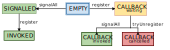
\includegraphics[width=\textwidth]{Cell_States.png}
  \caption{State transition diagram for a single cell.}
  \label{fig:cqs-cell-states}
\end{figure}

\subsection{Verification of Broadcast}
\label{sec:broadcast-spec}

In the following we describe the specifications we proved for the functions implemented in Eio's \ocamlin{Broadcast} module.
Note that all specifications obey the empty protocol because the code does not perform any effects.
For all three operations, the Eio implementation and specification differs from what is already verified in the original CQS (e.g. due to some reordered instructions or a different control flow).
However, the specifications of the underlying operations for manipulating cell pointers are modular enough to allow us to prove the new specifications for \ocamlin{Broadcast.create}, \ocamlin{Broadcast.register}, and \ocamlin{Broadcast.try_unregister}.

As for \ocamlin{Broadcast.signal_all}, Eio implements this function by atomically increasing the signal pointer by the number \(n\) of registered callbacks and then processing all \(n\) cells between the old and new pointer position.
Because of technical differences in handling these pointers between the original CQS implementation of the paper~\cite{koval2023cqs} and the broadcast implementation of Eio we opted to verify a different implementation of \ocamlin{Broadcast.signal_all}, that increments the signal pointer \(n\) times in a loop.
We argue this does not change the observable behaviors of the function since we ensure that it can only be called once.

\subsubsection{\ocamlin{Broadcast.create}}
\label{sec:broadcast-spec-create}

The only precondition to create a new broadcast is the proposition \(inv\_heap\_inv\).
This is a piece of ghost state defined by the Iris standard library that models invariant locations, which are locations that can always be read.
That means they cannot be explicitly deallocated and can only exist in a garbage-collected setting, like \ocf{}.
The implementation of the linked list uses this internally.

The function returns a broadcast instance \(bcst\), along with the persistent \(\gsIsBcst{}\; bcst\) proposition that shows the value actually is a broadcast.
We also obtain the unique resource \gssignal{}, which is held by the enclosing promise and allows calling the \ocamlin{Broadcast.signal_all} function once.

\[
  \inferrule[Spec-BroadcastCreate]
  {inv\_heap\_inv}
  {\ewp{create\; ()}{\bot}{bcst.\; \gsIsBcst{}\; bcst \ast \gssignal{}}}
\]

\subsubsection{\ocamlin{Broadcast.register}}
\label{sec:broadcast-spec-suspend}

% For a \emph{register} operation the \emph{suspend permit} from the original CQS is not needed anymore since we do the \emph{enqueue registration} internally.
A register operation takes a callback \(cb\) and the associated resource \(\gsIsCb{}\; cb\; R\) which represents the permission to invoke the callback.
We instantiate \(R\) with \gspdone{\gamma} so that the callback transports the knowledge that the promise has been fulfilled.
\(\gsIsCb{}\) is not persistent because the callback must be invoked only once.

\begin{align*}
  \gsIsCb{}\; cb\; R                            & \triangleq R \wand \ewp{cb\; ()}{\bot}{\top}                                                           \\
  \emph{isBroadcastRegisterResult}\; r\; cb\; R & \triangleq \begin{aligned}[t]
                                                  & (\ulcorner r = Invoked \urcorner)                                                           \\
                                                \vee\; & (\ulcorner r = Registered\; h \urcorner \ast \emph{isBroadcastRegisterHandle}\; h\; cb\; R) 
                                                \end{aligned}\\
  \emph{isBroadcastRegisterHandle}              & : Val \to Val \to iProp \to iProp
\end{align*}

The \ocamlin{Broadcast.register} function tries to insert a callback into the next cell designated by the register pointer.
If it succeeds the function returns a \ocamlin{Registered handle} value that can be used by \ocamlin{Broadcast.try_unregister}.
But if the cell is already in the \textbf{SIGNALLED} state, the function immediately invokes the callback and returns a \ocamlin{Invoked} value.

\[
  \inferrule[Spec-BroadcastRegister]
  { \gsIsBcst{}\; bcst \ast \gsIsCb{}\; callback\; R }
  { \ewp{register\; bcst\; callback}{\bot}{r.\; \emph{isBroadcastRegisterResult}\; r\; callback\; R}}
\]

\subsubsection{\ocamlin{Broadcast.try_unregister}}
\label{sec:broadcast-spec-cance}

Given a handle and its \(\textit{isBroadcastRegisterHandle}\; h\; cb\; R\) resource, \ocamlin{Broadcast.try_unregister} tries to cancel the registration of the callback.

If the callback had already been invoked by \ocamlin{Broadcast.signal_all} (i.e. the state is \(\textbf{CALLBACK}_\textbf{invoked}\)) the function returns \ocamlin{false} and no resources are returned to the caller.
Otherwise, the permission to invoke the callback \(\gsIsCb{}\; cb\) is returned.

\[
  \inferrule[Spec-BroadcastTryCancel]
  { \emph{isBroadcastRegisterHandle}\; h\; cb\; R }
  { \ewp{try\_unregister\; h}{\bot}{b.\; if\; b\; then\; \gsIsCb{}\; cb\; R\; else\; \top}}
\]

\subsubsection{\ocamlin{Broadcast.signal_all}}
\label{sec:broadcast-spec-signal-all}

To call \ocamlin{Broadcast.signal_all} the unique \(\gssignal{}\) resource is needed, along with a duplicable \(R\), so that it can be used to invoke multiple callbacks.
The function does not return any resources because its only effect is making an unknown number of fibers resume execution, which we cannot easily formalize in Iris.

\[
  \inferrule[Spec-BroadcastSignalAll]
  { \gsIsBcst{}\; bcst \ast \always R \ast \gssignal{}}
  { \ewp{signalAll\; bcst}{\bot}{\top} }
\]

\subsection{Changes from the Original CQS}
\label{sec:broadcast-spec-removed-features}

The original CQS supports multiple additional features like a synchronous mode for suspend and resume, and also a smart cancellation mode.
These features enlarge the state space of CQS and complicate the verification but are not used in Eio so when we ported the verification of CQS to our Eio development we removed support for these features.
This reduced the state space of a cell shown in figure~\ref{fig:cqs-cell-states-original} to a more manageable size when adapting the proofs.

\begin{figure}[ht]
  \includegraphics[width=\textwidth]{Cell_States_Original.png}
  \caption{Cell states in the original CQS from~\cite{koval2023cqs} (page 42).}
  \label{fig:cqs-cell-states-original}
\end{figure}

The part of the verification of the original CQS that we had to customize for Eio was originally 3600 lines of Coq code but -- due to these simplifications -- we could reduce it by approximately 1300 lines of Coq code.
Additionally, there are ~4000 lines of Coq code about lower-level functionality that we did not need to adapt when porting them to our development.

% The number of active cells \(n\) (i.e. the length of the queue) is tracked by the logical resource \(CQSState\; n\).
% In normal usage of CQS, the atomic variable of the outer synchronization construct would encode the length of the queue in its value and keep this resource in an associated invariant.
% Changing the length of the queue is done using \emph{enqueue} and \emph{dequeue registration} logical operations when opening this invariant.

% However, for promises the exact length of the queue is irrelevant because the \emph{signalAll} operation will always set the length to 0.
% So in the adapted proof for Eio's broadcast we keep the \(CQSState\; n\) resource in the invariant of the broadcast itself.
% As a consequence we also move the \emph{enqueue} and \emph{dequeue registration} out of the public logical API because they are now done internally.


\section{Adding Support for Thread-Local Variables}
\label{sec:thread-local-vars}

% General information about the GetContext effect and that it's used to implement thread-local variables

So far we have looked at a protocol \(\proto{2}\) that has two effects which suffice to model fibers that can suspend and fork off new fibers.
But fibers in Eio can use an additional effect called \egetctx{} that we discuss in this section.
For each fiber the scheduler keeps track of context metadata, one part of which are \emph{thread-local variables}.
Thread-local variables are state that is shared between all fibers of one scheduler (hence thread-local) and a fiber gets access to them via the \egetctx{} effect.

% Example of how thread-local variables can be used for a tracing log.

Since all fibers of one scheduler execute concurrently on one system-level thread, they have exclusive access to the thread-local variables while they are running.
This allows a practical form of shared state without the overhead of synchronization primitives of multithreaded data structures.
Two example use-cases are per-scheduler tracing of events, where all fibers of one scheduler write to a common log,
and inter-fiber message passing, where fibers use a simple queue to exchange messages.
Of course, this comes with the restriction that it is only usable for fibers running in the same thread.

% What we want to verify about thread-local variables. 

In Eio thread-local variables are represented by a dictionary from variable names to arbitrary values and expose an intended API that only allows adding new entries.
However, it is still possible for fibers to arbitrarily modify the whole dictionary, so for demonstration purposes we model thread-local variables as a single mutable reference that is part of the context record: \ocamlin{ctx.tlv}.
Properties we want to prove about thread-local variables are:
\begin{enumerate}
    \item Each time a fiber performs a \egetctx{} effect it receives the same reference.
    \item As long as a fiber does not perform other effects like \efork{} or \esuspend{}, it holds exclusive ownership of the reference.
\end{enumerate}

Code examples illustrating the properties are shown in figure~\ref{fig:tlv-example}.
Note that these are only the most basic properties showing that \ocamlin{ctx.tlv} acts like a normal reference, but one that can be accessed via an effect.
To enable modular proofs of concrete fibers using thread-local variables, we include in our logical definition a predicate \(T\) on the stored value that can be instantiated by fibers as needed.

\begin{figure}[ht]
    \begin{minted}{ocaml}
let fiber1 () =
  let ctx = perform (GetContext ()) in
  let ctx2 = perform (GetContext ()) in
  assert (ctx.tlv == ctx2.tlv)

let fiber2 () =
  let ctx = perform (GetContext ()) in
  let v = !ctx.tlv in
  (* some computation that does not perform Fork/Suspend *)
  ...
  assert (!ctx.tlv == v)
  \end{minted}
    \caption{Constructed example of safety for thread-local variables.}
    \label{fig:tlv-example}
\end{figure}

\subsection{Changes to Logical State}

% How do we extend the protocol and change the logical definitions.
To handle thread-local variables in our development we must change both the implementation and logical definitions.
The necessary changes to the implementation are trivial, so we just refer to the mechanization\footnote{TODO insert link}.
The new definitions are described in figure~\ref{fig:logical-state-ext}.
\(\gsTLVAg{}\; \delta\; tlv\) is used to show the uniqueness of the location \(tlv\).
\(\gsIsFiberContext{}\; \delta\; tlv\) represents the context that is tracked for each fiber, where \(\delta\) is a shorthand for multiple ghost names.
It expresses that the location \(tlv\) is a thread-local variable which maps to some value \(v\) satisfying \(T\).
The predicate T is hidden behind a \(\gsSavedPred{}\) indirection to make the mechanization easier.
\(\gsFiberResources{}\; \delta\) is then used to abstract away the concrete location \(tlv\).
This predicate represents all resources that a fiber owns while it is running, so each fiber specification now has this as a precondition.
Finally, we must change the definition of \(\gsReady{}\) to require \(\gsFiberResources{}\) as a precondition because it is needed to invoke the continuations saved in the scheduler's run-queue.

\begin{figure}[ht]
    \begin{align*}
        \gsTLVAg{}\; \delta\; tlv \triangleq\;            & \ownGhost{\delta}{agree(tlv)}  \qquad \textrm{Persistent}(\gsTLVAg{\delta}{tlv})                          \\
        \gsIsFiberContext{}\; \delta\; tlv\; \triangleq\; & \gsTLVAg{}\; \delta\; tlv \ast \exists T\; v.\; tlv \mapsto v \ast \gsSavedPred{}\; \delta\; T \ast T\; v \\
        \gsFiberResources{}\; \delta\; \triangleq\;       & \exists\; tlv.\; \gsIsFiberContext{}\; \delta\; tlv\;                                                     \\
        \gsReady{}\; \delta\; f \triangleq\;              & \gsFiberResources{}\; \delta\; \wand{} \ewp{f\; ()}{\bot}{\top}
    \end{align*}
    \caption{Logical state definitions for the verification of our Eio model.}
    \label{fig:logical-state-ext}
\end{figure}

The effect protocols of \efork{} and \esuspend{} are amended so that they pass \(\gsFiberResources{}\) from a fiber to the scheduler and from there to the next running fiber via the protocol pre- and postconditions as shown in figure~\ref{fig:coop-protocol-ext}.
The \efork{} effect now also passes the concrete reference that should be used as the thread-local variable of the new fiber.
A fiber uses the \egetctx{} effect to receive the fiber context value and a copy of \(\gsTLVAg{}\).
This is used to show that the reference \(ctx.tlv\) is equal to the one from \(\gsFiberResources{}\) that the fiber already owns so that the contained points-to predicate can be used.

The crux is that now the protocol \proto{} is parameterized by the ghost name \(\delta\) that identifies the thread-local variable.
This so that both the fiber and the scheduler agree on this ghost name.

\begin{figure}[ht]
    \begin{equation*}
        \proto{}~\delta \triangleq \begin{aligned}[t]
            Fork\;       & \#\; \begin{aligned}[t]
                                     & !\; tlv\; e\; ((tlv, e))\; \begin{aligned}[t]
                                                   & \big\{ \gsFiberResources{}\; \delta\; T \ast \gsTLVAg{}\; \delta\; tlv\; \ast                              \\
                                                   & \later\; (\gsFiberResources{}\; \delta\; T \wand{} \ewp{e}{Coop}{\gsFiberResources{}\; \delta\; T}) \big\}
                                              \end{aligned} . \\
                                     & ?\; ()\; \{ \gsFiberResources{}\; \delta\; T \}
                                \end{aligned}                                 \\
            Suspend\;    & \#\; \begin{aligned}[t]
                                     & !\; reg\; W\; (reg)\; \{\gsFiberResources{}\; \delta\; T \ast \gsIsReg{}\; reg\; W\}. \\
                                     & ?\; y\; (y)\; \{ \gsFiberResources{}\; \delta\; T \ast W\; y \}
                                \end{aligned} \\
            GetContext\; & \#\; !\; ()\; \{\top\}.\; ?\; ctx\; (ctx)\; \{ \gsTLVAg{}\; \delta\; ctx.tlv \}
        \end{aligned}
    \end{equation*}
    \caption{Definition of extended \proto{} protocol with \efork{}, \esuspend{}, and \egetctx{} effects.}
    \label{fig:coop-protocol-ext}
\end{figure}

These changes suffice to prove the safety of the two examples in figure~\ref{fig:tlv-example}.


\section{Evaluation}
\label{sec:evaluation}
We evaluate our model of Eio on a simple example program that uses all features supported by our implementation.
The example program (shown in figure~\ref{fig:eval_code}) may look contrived since it does not do any "useful" computation, but the value of Eio as a library comes from composing computations -- not in what is computed concretely.

The program's \ocamlin{main_fiber} function forks off a new fiber \ocamlin{dispatch} (line~\ref{ln:eval_dispatch}) and communicates with it over a one-element channel represented by the thread-local variable.
The channel is initially empty (first argument to \ocamlin{Scheduler.run} in line~\ref{ln:eval_none}) and \ocamlin{dispatch} polls for data (line~\ref{ln:eval_wait}).
\ocamlin{main_fiber} sends one integer \ocamlin{data} (lines~\ref{ln:eval_receive},\ref{ln:eval_send}) to \ocamlin{dispatch} which will then run two copies of \ocamlin{(work data)} (line~\ref{ln:eval_thread}) in separate threads, and sum their results.
The \ocamlin{work} function simulates time passing using the \ocamlin{yield} function (line~\ref{ln:eval_work}) and returns its first argument.
Yield performs a \esuspend{} effect but calls the \ocamlin{waker} function immediately, which has the effect of placing the current fiber at the back of the scheduler's run queue to give other fibers a chance to run.

The example program therefore uses the basic functions for forking and awaiting the completion of fibers, multiple schedulers running in different threads, as well as thread-local variables to communicate between fibers within one thread.

\begin{figure}[ht]
    \begin{minted}[escapeinside=@@]{ocaml}
let yield () = @\label{ln:eval_yield}@ 
  perform (Suspend (fun waker -> waker ()))

let work x () = 
  yield (); @\label{ln:eval_work}@
  x

let rec wait_for_data (tlv : tlv ref) =
  match !tlv with
  | None -> yield (); wait_for_data tlv
  | Some data -> tlv := None; data @\label{ln:eval_receive}@

let dispatch () =
  let tlv = perform (GetContext ()) in
  let data = wait_for_data tlv in @\label{ln:eval_wait}@
  let p1 = Fiber.fork_promise (fun () -> Domain_manager.new_scheduler (work data)) in @\label{ln:eval_thread}@
  let p2 = Fiber.fork_promise (fun () -> Domain_manager.new_scheduler (work data)) in
  let r1 = Promise.await p1 in
  let r2 = Promise.await p2 in
  r1 + r2

let main_fiber data () =
  let p = Fiber.fork_promise dispatch in @\label{ln:eval_dispatch}@
  let tlv = perform (GetContext ()) in
  tlv := Some data; @\label{ln:eval_send}@
  Promise.await p

let main () = 
  Scheduler.run None (main_fiber 21) @\label{ln:eval_none}@
\end{minted}
    \caption{Example program to use all implemented features.}
    \label{fig:eval_code}
\end{figure}

We first give the final specifications of the most important components of our model library in figure~\ref{fig:eval-total}.
The specifications contain both extensions we discussed in sections~\ref{sec:domain-manager} and~\ref{sec:thread-local-vars}.

\begin{figure}[ht]
    \begin{align*}
        \gsReadyF{}~l~\Omega~\gamma~q~k & \triangleq \begin{aligned}[t]
                                                         & \gsFiberResources{l}{\Omega} \wand                                                                                                           \\
                                                         & \later isQueueReader~q~(\gsReadyF{}~l~\Omega~\gamma~q) \wand                                                                                  \\
                                                         & \quad \ewp{k~()}{\bot}{\_.\; \gsFiberResources{l}{\Omega} \ast \later isQueueReader~q~(\gsReadyF{}~l~\Omega~\gamma~q) \ast \gspdone{\gamma} }
                                                    \end{aligned} \\
        \gsIsWaker{}~wkr~W             & \triangleq \forall v.   \;  W\; v \wand{} \ewp{wkr\ \ v}{\bot}{\top}                                                                                                \\
        \gsIsRegF{}~reg~W~S             & \triangleq \forall wkr. \; \gsIsWaker{}\; wkr\; W \wand{} \ewp{reg\ \ wkr}{\bot}{\always S}                                                                         \\
        \protoF{}~l_{tlv}~\Omega              & \triangleq \begin{aligned}[t]
                                                        Fork\;       & \#\; \begin{aligned}[t]
                                     & !\; e\; (e)\; \begin{aligned}[t]
                                           & \big\{ \gsFiberResources{l_{tlv}}{\Omega} \ast                                                                              \\
                                           & \later\; (\gsFiberResources{l_{tlv}}{\Omega} \wand{} \ewp{e\ \ ()}{\protoF{}~l_{tlv}~\Omega}{\gsFiberResources{l_{tlv}}{\Omega}}) \big\} .
                                      \end{aligned} \\
                                     & ?\; ()\; \{ \gsFiberResources{l_{tlv}}{\Omega} \}
                                \end{aligned}                                             \\
                                                        Suspend\;    & \#\; \begin{aligned}[t]
                                     & !\; reg\; W\; S\; (reg)\; \{\gsFiberResources{l_{tlv}}{\Omega} \ast \gsIsRegF{}\; reg\; W\; S\}. \\
                                     & ?\; v\; (v)\; \{ \gsFiberResources{l_{tlv}}{\Omega} \ast W~v \ast S \}
                                \end{aligned} \\
                                                        GetContext\; & \#\; !\; ()\; \{\top\}.\; ?\; (l_{tlv})\; \{ \top \}
                                                    \end{aligned}
    \end{align*}
    \begin{mathpar}
        \inferrule[Spec-Run]
        { \Omega~init \;\ast \\\\ \forall l_{tlv}.\; \gsFiberResources{l_{tlv}}{\Omega} \wand \ewp{main\ \ ()}{\protoF{}~l_{tlv}~\Omega}{v.\; \always \Phi~v \ast \gsFiberResources{l_{tlv}}{\Omega}} }
        { \ewp{run\ \ init\ \ main}{\bot}{v.\; \always \Phi~v \ast \gsFiberResources{l_{tlv}}{\Omega}} }
        %
        \and
        %
        \inferrule[Spec-ForkPromise]
        { \gsPInv{} \ast \gsFiberResources{l_{tlv}}{\Omega} \;\ast \\\\ \gsFiberResources{l_{tlv}}{\Omega} \wand \ewp{f\ \ ()}{\protoF{}~l_{tlv}~\Omega}{v.\; \always \Phi~v \ast \gsFiberResources{l_{tlv}}{\Omega}} }
        { \ewp{fork\_promise\ \ f}{\protoF{}~l_{tlv}~\Omega}{p.\; \gsIsPr{}~p~\Phi \ast \gsFiberResources{l_{tlv}}{\Omega}} }
        %
        \and
        %
        \inferrule[Spec-Await]
        { \gsPInv{} \ast \gsFiberResources{l_{tlv}}{\Omega} \ast \gsIsPr{}~p~\Phi }
        { \ewp{await\ \ p}{\protoF{}~l_{tlv}~\Omega}{p.\; \gsIsPr{}~p~\Phi \ast \gsFiberResources{l_{tlv}}{\Omega}} }
        %
        \and
        %
        \inferrule[Spec-NewScheduler]
        { \Omega'~init \;\ast \\\\ \forall l'_{tlv}.\; \gsFiberResources{l'_{tlv}}{\Omega} \wand \ewp{main\ \ ()}{\protoF{}~l'_{tlv}~\Omega'}{v.\; \always \Phi~v \ast \gsFiberResources{l'_{tlv}}{\Omega'}} }
        { \ewp{new\_scheduler\ \ init\ \ main}{\protoF{}~l~\Omega}{v.\; \always \Phi~v \ast \gsFiberResources{l}{\Omega}} }
    \end{mathpar}

    \caption{Specification of the public interface of the Eio library model.}
    \label{fig:eval-total}
\end{figure}

Using these specifications we proved the safety of the example program and its functional correctness by establishing specifications for each function as shown in figure~\ref{fig:eval-spec}.
We can see that there is some amount of boilerplate (colored in {\color{blue} blue}).
Each function that yields execution to another fiber by performing an effect -- either directly or indirectly through another function call -- needs \({\color{blue}\gsFiberResources{l_{tlv}}{\Omega}}\), which signifies the ownership over the thread-local variable.
Additionally, any fiber that wants to fork off another fiber using \ocamlin{Fiber.fork_promise} needs the persistent \({\color{blue}\gsPInv{}}\) resource to interact with the global collection of promises.
The predicate \(\Omega_{chan}~\gamma\) as part of \(\gsFiberResources{l_{tlv}}{(\Omega_{chan}~\gamma)}\) restricts the thread-local variable \(l_{tlv}\) to be a channel for a single message \(n\).

\begin{figure}[ht]
    \begin{align*}
        \Omega_{chan}~\gamma~v & \triangleq \begin{aligned}[t]
                                                       & \ulcorner v = None \urcorner                                                    \\[-5pt]
                                                \vee\; & \exists n.\; \ulcorner v = Some~n \urcorner \ast \ownGhost{\gamma}{\aginj{}(n)}
                                            \end{aligned} \\
    \end{align*}
    \begin{mathpar}
        \inferrule[Spec-Work]
        { {\color{blue}\gsFiberResources{l_{tlv}}{\Omega}} }
        { \ewp{work\ \ n\ \ ()}{\protoF{}~l_{tlv}~\Omega}{v.\; \ulcorner v = n \urcorner \ast {\color{blue}\gsFiberResources{l_{tlv}}{\Omega}}} }
        %
        \and
        %
        \inferrule[Spec-WaitForData]
        { {\color{blue}\gsFiberResources{l_{tlv}}{(\Omega_{chan}~\gamma)}} }
        { \ewp{wait\_for\_data\ \ l}{\protoF{}}{v.\; \exists n.\; \ulcorner v = n \urcorner \ast \ownGhost{\gamma}{\aginj{}(n)} \ast {\color{blue}\gsFiberResources{l_{tlv}}{(\Omega_{chan}~\gamma)}}} }
        %
        \and
        %
        \inferrule[Spec-Dispatch]
        { {\color{blue}\gsPInv{}} \ast {\color{blue}\gsFiberResources{l_{tlv}}{(\Omega_{chan}~\gamma)}} }
        { \ewp{dispatch\ \ ()}{\protoF{}}{v.\; \exists n.\; \ulcorner v' = n + n \urcorner \ast \ownGhost{\gamma}{\aginj{}(n)} \ast {\color{blue}\gsFiberResources{l_{tlv}}{(\Omega_{chan}~\gamma)}}} }
        %
        \and
        %
        \inferrule[Spec-MainFiber]
        { {\color{blue}\gsPInv{}} \ast {\color{blue}\gsFiberResources{l_{tlv}}{(\Omega_{chan}~\gamma)}} \ast \ownGhost{\gamma}{\aginj{}(n)} }
        { \ewp{main\_fiber\  n\  ()}{\protoF{}}{v.\; \ulcorner v = n + n \urcorner \ast {\color{blue}\gsFiberResources{l_{tlv}}{(\Omega_{chan}~\gamma)}}} }
        %
        \and
        % 
        \inferrule[Spec-Main]
        { }
        { \ewp{main\ \ ()}{\bot}{v.\; \ulcorner v = 42 \urcorner} }
    \end{mathpar}
    \caption{Specification of the example program.}
    \label{fig:eval-spec}
\end{figure}

While we proved the safety of this program (and of the core abstractions of the Eio library), the complete Eio library has more features that are still unexplored.
This includes cancellation of fibers, resource management using switches and several operating system primitives like timers, so we cannot make any statements about programs using these features.
Nevertheless, our model is an important step in the direction of proving the safety of Eio and programs that use it.
Iris along with its features like ghost state and shareable invariants to reason about multithreaded and stateful code were key in this development.


\section{Conclusion}
\label{sec:conclusion}

\subsection{Related Work}
\paragraph*{Concurrency With Effects}
There are other approaches to implementing cooperative concurrency with effects even within \ocf{}.
One example is the Picos framework~\cite{Picos}, an interoperability framework that defines a small set of data types and effects that can be reused by other cooperative concurrency libraries (such as Eio)
in order to speak a common protocol and be mutually interoperable.
Picos defines \emph{computations} and \emph{fibers}, which are mostly equivalent, respectively, to Eio's promises and fibers.
The main difference is the \emph{trigger} concept, which in Eio's terms can be thought of as a mutable reference to an optional \ocamlin{waker} function.
% The workflow to await a result in Eio is to, first define a \ocamlin{register} function and perform a \esuspend{} effect with it. 
% The scheduler will call the \ocamlin{register}
The workflow to await a future result (i.e. a Picos computation) resembles Landin's Knot in that it consists of first attaching an empty trigger to the computation and then assigning a \ocamlin{waker} function later.
This is done by performing an \emph{Await} effect after attaching the trigger so that the effect handler (implemented by a library such as Eio) then creates a \ocamlin{waker} function and assigns it to the trigger.
When the computation finishes it will signal the trigger, which calls the \ocamlin{waker} function and consequently places the original fiber in the scheduler's run queue.

While the \emph{Await} effect carrying a trigger is technically first-order -- as opposed to Eio's higher-order \esuspend{} effect carrying a \ocamlin{register} function --
a trigger still contains higher-order state.
So it is unclear to us whether a specification for the Picos primitives would be any simpler to prove or easier to use than the specification for Eio primitives we have presented so far.

\paragraph*{Session Types as Effect Specifications}
Protocols in \hazel{} take some inspiration from session types but with the restriction that a protocol is always an infinite repetition of a single step, whereas session types usually allow defining a sequence of different steps.
Current work by Tang~\cite{tangeff} explores the connection between session types and effect protocols further and defines a lambda calculus \(\lambda^{\mbox{{\footnotesize \Letter}}}_{\mathrm{eff}}\) that uses a standard session type formalization
for its effect system.
This allows a programmer to define multistep protocols and even bidirectional effects where the handler and client swap roles.
However, for our purposes \hazel{} is completely sufficient since multistep protocols can be simulated by \hazel{}'s protocols and bidirectional effects are not possible in \ocf{} to begin with.

% \paragraph*{}
% Current work by van Rooij~\cite{?} extends the type and effects system Tes of de Vilhena~\cite{de2022proof} to track in the type system whether a continuation is one- or multi-shot.

% \paragraph*{Other Verifications of Eio Primitives}
% \todo{There seems to be something called zebre that is referenced by Eio and implements at least the Lf\_queue of Eio \url{https://github.com/clef-men/zebre/} but otherwise appears to model a different kind of scheduler.}

\subsection{Future Work}
The work we presented so far suffices to prove the safety of programs that use a small subset of the full functionality provided by Eio.
To improve the usefulness of our model and be applicable to more programs it would be desirable to incorporate more features into our model of Eio in future work, such as switches and support for cancelling fibers.
While switches are mainly used for a hierarchical organization of fibers and to efficiently clean up fiber resources, cancellation poses some interesting safety questions because there are situations that must be avoided, such as being able to cancel a fiber twice.

Instead of growing the model of Eio it would also be interesting to extend the existing specifications.
Mainly, we would be interested in proving that a scheduler will never "forget fibers".
Since weakest preconditions in Iris do not prove termination our specifications have the unfortunate drawback of being fulfilled by functions that diverge.
Because a scheduler explicitly handles fiber continuations it would be possible to accidentally drop a continuation which has the effect of making the fiber diverge, as well as any other fiber that awaits its result.

While we cannot solve the whole termination problem (since deadlocks are possible), intuitively we should be able to track the state of each fiber to ensure that when a fiber is captured in a continuation,
the continuation is used linearly, which means that it is explicitly invoked or discarded at some point.
This also extends to data structures that contain continuations like the scheduler's run queue and a broadcast, as they must never drop the contained continuations.
To track the linear usage of continuations it could be helpful to draw inspiration from Iron~\cite{bizjak2019iron}, a separation logic built on Iris to enable reasoning about linear resources.

% Finally, to make the statement "the program can diverge but not due to mishandled continuations" formal, it might be possible to use Transfinite Iris~\cite{spies2021transfinite} and prove a \emph{termination-preserving refinement} 
% of the scheduler to a simpler scheduler where the linear handling of fiber continuations is more easily provable.
% However, it is non-obvious how such a simpler scheduler would look like since termination of the whole program 

\subsection{Results}

In this thesis we have proven specifications for a subset of the Eio library, including a common denominator scheduler that controls fibers which can await the completion of promises in a multithreaded setting.
We have also defined and verified general and reusable protocols for the main three effects of Eio: \efork{}, \esuspend{}, and \egetctx{}.
We showed that the function specifications and the effect protocols are enough to verify the safety (including effect safety) of an example program that uses all of our modelled features.
Additionally, we have verified specifications for two nontrivial data structures used by Eio.
For the broadcast data structure we adapted the existing proof of CQS by Koval et al.~\cite{koval2023cqs}
and for the scheduler's run queue we proved a -- to our knowledge novel -- specification for a multi-producer single-consumer queue with a temporarily suspendable invariant.
Finally, we have extended the original \hazel{} language with multithreading primitives and amended the adequacy result which shows that we can use this language to reason about programs that use both multithreading and effect handlers.


% from https://tex.stackexchange.com/a/174628
\appendix
\addcontentsline{toc}{section}{Appendix}
\section*{Appendix}
\label{sec:appendix}

\renewcommand{\thesubsection}{\Alph{subsection}}

\subsection{Translation Table}
\label{sec:apdx-translation}

\begin{table}[ht]
  \begin{tabular}{l|l|l}
    Eio                          & Thesis                       & Mechanization          \\
    \hline
    \ocamlin{enqueue}            & \ocamlin{waker} function     & \ocamlin{waker}        \\
    \ocamlin{f}                  & \ocamlin{register} function  & \ocamlin{register}     \\
    \ocamlin{Fiber.fork_promise} & \ocamlin{Fiber.fork_promise} & \ocamlin{fork_promise} \\
    \ocamlin{Promise.await}      & \ocamlin{Promise.await}      & \ocamlin{await}        \\
    \ocamlin{Sched.run}          & \ocamlin{Scheduler.run}      & \ocamlin{run}          \\
  \end{tabular}
\end{table}

\subsection{Towards A multithreaded Scheduler}
\label{sec:apdx-mt}

OCaml 5 added not only effect handlers but also the ability to use multiple threads of execution, which are called \emph{domains} (in the following we use the terms interchangeably).
Each domain in OCaml 5 corresponds to one system-level thread and the usual rules of multithreaded execution apply, i.e. domains are preemtively scheduled and can share memory.
Eio defines an operation to make use of multi-threading by forking off a new thread and running a separate scheduler in it.
So while each Eio scheduler is only responsible for fibers in a single thread, fibers can await and communicate with fibers running in other threads.

In order for a fiber to be able to await fibers in another thread, the \ocamlin{wakers_queue} [note it will be in the Simple Scheduler section] from above is actually a thread-safe queue based on something called CQS, which we will discuss in detail in a later section.

Heaplang supports reasoning about multithreaded programs by implementing fork and join operations for threads and defining atomic steps in the operational semantics, which enables the use of Iris \emph{invariants}.
In contrast, \hazel{} did not define any multithreaded operational semantics but it contained most of the building blocks for using invariants.
In the following we explain how we added a multithreaded operational semantics and enabled the use of invariants.

% \ocamlin{}`
% Aside: Memory Model in OCaml 5
% In the OCaml 5 memory model, \emph{atomic variables} are needed in order to access shared memory without introducing data races.
% Instead of modelling atomic variables in \hazel{}, we continue to use normal references because the multithreaded operational semantics by definition defines all memory operations to be sequentially consistent. This seems to be the standard approach and is done the same way in Heaplang.
% \ocamlin{}`

\subsubsection*{Adding Invariants to \hazel{}}

Invariants in Iris are used to share resources between threads.
They encapsulate a resource to be shared and can be opened for a single atomic step of execution.
During this step the resource can be taken out of the invariant and used in the proof but at the end of the step the invariant must be restored.

\hazel{} did already have the basic elements necessary to support using invariants.
It defined a ghost cell to hold invariants and proved an invariant access lemma which allows opening an invariant if the current expression is atomic.
In order to use invariant we only had to provide proofs for which evaluation steps are atomic.
We provided proofs for all primitive evaluation steps.
The proofs are the same for all steps so we just explain the one for \ocamlin{Load}.

\begin{minted}{coq}
Lemma ectx_language_atomic a e :
head_atomic a e → sub_exprs_are_values e → Atomic a e.

Instance load_atomic v : Atomic StronglyAtomic (Load (Val v)).
Instance store_atomic v1 v2 : Atomic StronglyAtomic (Store (Val v1) (Val v2)).
...
\end{minted}

An expression is atomic if it takes one step to a value, and if all subexpressions are already values.
The first condition follows by definition of the step relation and the second follows by case analysis of the expression.

Since performing an effect starts a chain of evaluation steps to capture the current continuation, it is not atomic.
For the same reason an effect handler and invoking a continuation are not atomic except in degenerate cases.
Therefore, invariants and effects do not interact in any interesting way.
\todo{How we add support for the iInv tactic to use invariants more easily.}

\subsubsection*{Adding Multi-Threading to \hazel{}}

To allow reasoning in \hazel{} about multithreaded programs we need a multithreaded operational semantics as well as specifications for the new primitive operations \efork{}, \ocamlin{Cmpxcgh} and \ocamlin{FAA}.

The language interface of Iris provides a multithreaded operational semantics that is based on a thread-pool.
The thread-pool is a list of expressions that represents threads running in parallel.
At each step, one expressions is picked out of the pool at random and executed for one thread-local step.
Each thread-local step additionally returns a list of forked-off threads, which are then added to the pool.
This is only relevant for the \efork{} operation as all other operations naturally don't fork off threads.

% (e, \sigma) ->_t (e', \sigma', es')
% ------------------------------------------------------------
% (es_1 ++ e ++ es_2, \sigma) ->_mt (es_1 ++ e' ++ es_2 + es', \sigma')

Heaplang implements multi-threading like this and for \hazel{} we do the same thing.
We adapt \hazel{}'s thread-local operational semantics to include \efork{}, \ocamlin{Cmpxchg} and \ocamlin{FAA} operations and to track forked-off threads and get a multithreaded operational semantics "for free" from Iris' language interface.

Additionally, we need to prove specifications for these three operations.
\ocamlin{Cmpxchg} and \ocamlin{FAA} are standard so we will not discuss them here.
The only interesting design decision in the case of \hazel{} is how effects and \efork{} interact.
This decision is guided by the fact that in OCaml 5 effects never cross thread-boundaries.
An unhandled effect just terminates the current thread.
As such we must impose the empty protocol on the argument of \efork{}.

% EWP e <| \bot |> { \top }
% -------------------------------------
% EWP (Fork e) <| \Phi |> { x, x = () }

Using these primitive operations we can then build the standard \ocamlin{CAS}, \ocamlin{Spawn}, and \ocamlin{Join} operations on top and prove their specifications.
For \ocamlin{Spawn} \& \ocamlin{Join} we already need invariants as the point-to assertion for the done flag must be shared between the two threads.

% Lemma spawn_spec (Q : val → iProp Σ) (f : val) :
% EWP (f #()) <| \bot |> {{ Q }} -∗ EWP (spawn f) {{ v, ∃ (l: loc), ⌜ v = #l ⌝ ∗ join_handle l Q }}.

% Lemma join_spec (Q : val → iProp Σ) l :
% join_handle l Q -∗ EWP join #l {{ v, Q v }}.

% Definition spawn_inv (γ : gname) (l : loc) (Q : val → iProp Σ) : iProp Σ :=
% ∃ lv, l ↦ lv ∗ (⌜lv = NONEV⌝ ∨
% ∃ w, ⌜lv = SOMEV w⌝ ∗ (Q w ∨ own γ (Excl ()))).

% Definition join_handle (l : loc) (Q : val → iProp Σ) : iProp Σ :=
% ∃ γ, own γ (Excl ()) ∗ inv N (spawn_inv γ l Q).

Note that for \ocamlin{Spawn} we must also impose the empty protocol on \ocamlin{f} as this expression will be forked-off.

This allows us to implement standard multithreaded programs which also use effect handlers.
For example, we can prove the specification of the function below that is based on an analogous function in Eio which forks a thread and runs a new scheduler inside it.
Note that same as in Eio the function blocks until the thread has finished executing, so it should be called in separate fiber.

% Definition spawn_scheduler : val :=
% (λ: "f",
% let: "new_scheduler" := (λ: <>, run "f") in
% let: "c" := spawn "new_scheduler" in
% join "c")%V.

% Lemma spawn_scheduler_spec (Q : val -> iProp Σ) (f: val) :
% promiseInv -∗ EWP (f #()) <| Coop |> {{ _, True }} -∗
% EWP (spawn_scheduler f) {{ _, True }}.

The scheduler \ocamlin{run} and therefore also the \ocamlin{spawn_scheduler} function don't have interesting return values, so this part of the specification is uninteresting.
What is more interesting is that they encapsulate the possible effects the given function \ocamlin{f} performs.

\subsection{A Note on Cancellation}
\label{sec:apdx-cancellation}

\begin{itemize}
  \item That we tried to model cancellation but the feature is too permissive to give it a specification.
  \item There is still an interesting question of safety (fibers cannot be added to a cancelled Switch).
  \item But including switches \& cancellation in our model would entail too much work so we leave it for future work.
\end{itemize}


\printbibliography

\end{document}